\section{Conclusion}

This project evaluated the knowledge capabilities of three advanced AI models, ChatGPT, Gemini, and Meta AI, by analyzing
their answers to questions generated from NotebookLM with the seminar transcript as source. The results revealed that
Gemini performed the best, achieving an accuracy of 96.75\%, followed by ChatGPT at 87.5\%, and Meta AI at 85\%. 
These findings highlight the strong baseline knowledge of all three AIs, with Gemini demonstrating exceptional accuracy.
\begin{figure}[H]
    \centering
    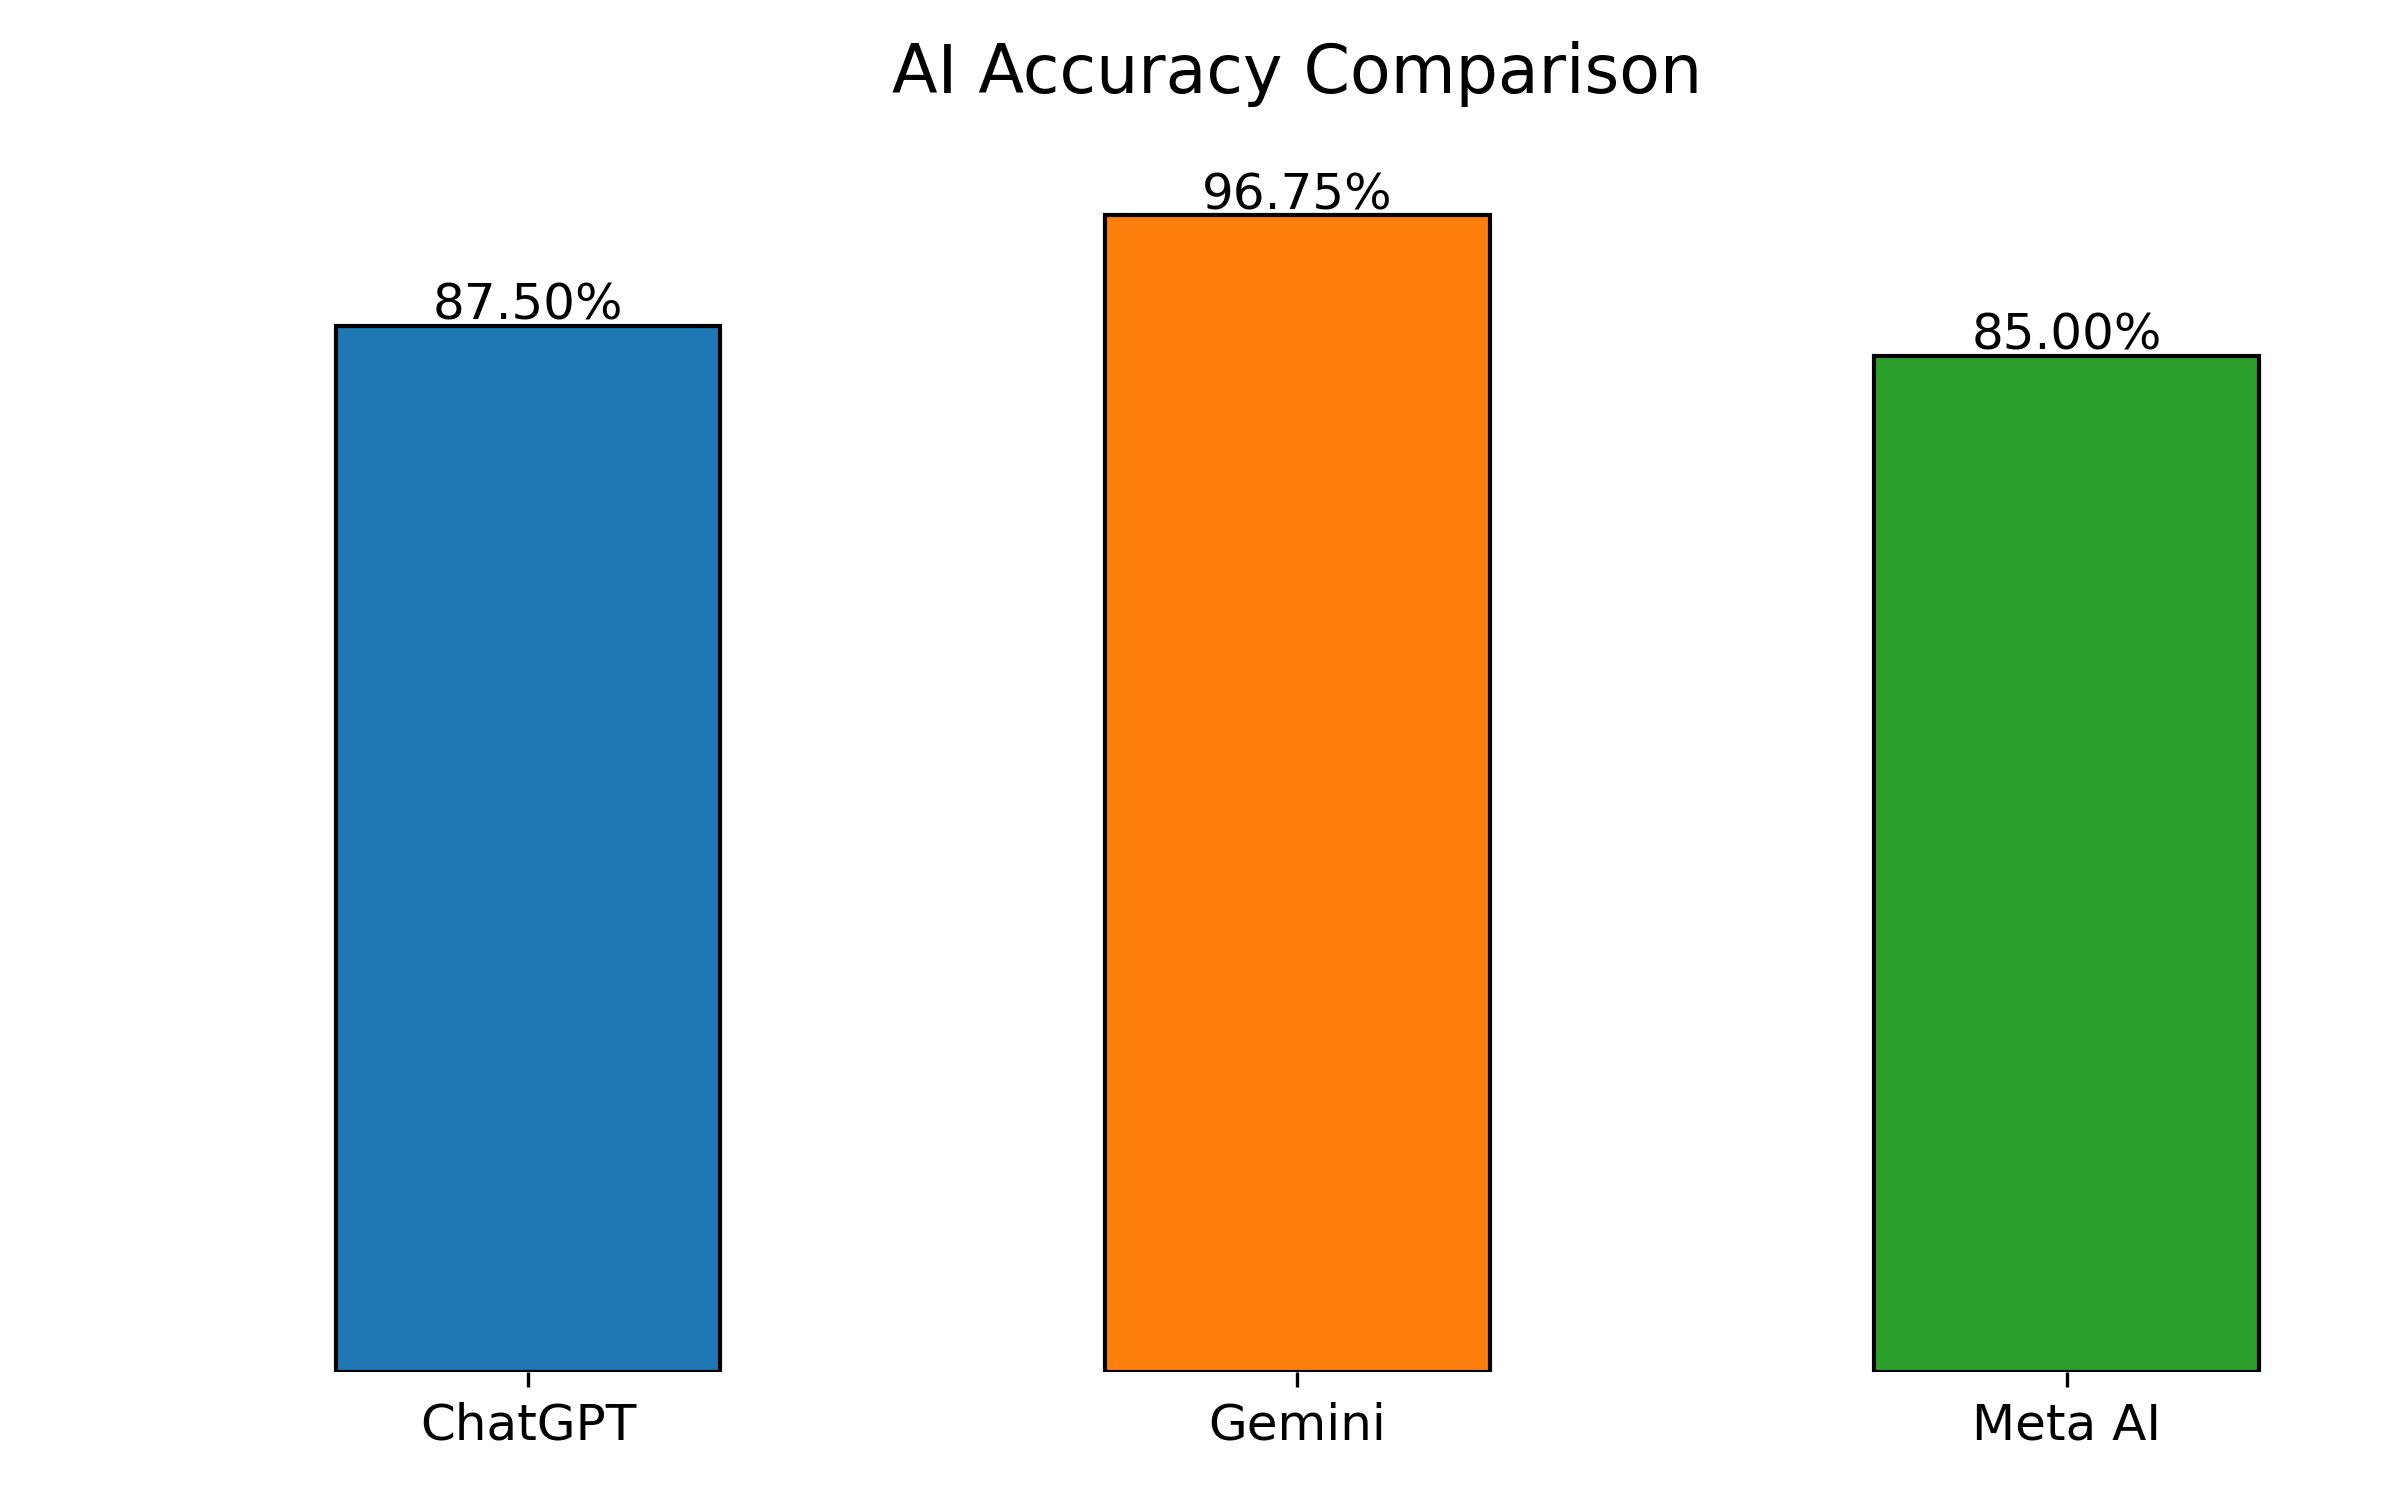
\includegraphics[scale=0.75]{Imagens/graph.jpg}
    \caption{Graph comparing the accuracy of the AIs}
\end{figure}
A notable challenge in the evaluation process was the use of NotebookLM. While it offered a structured way to assess
responses, its evaluation criteria were inconsistent, often changing between questions. For example, NotebookLM 
frequently marked answers as partially correct if specific details mentioned in the seminars were omitted, even when the 
broader context was accurate. Manual analysis showed that most of these flagged answers were actually correct, 
indicating that the evaluation process was overly strict and sometimes misleading.

The results prompt an important question: can these AI models replace traditional seminars, or are they better suited as
supplemental tools? While the high accuracy of their answers demonstrates a deep baseline knowledge, 
it is crucial to note that AI responses are limited to their pre-trained data and reasoning algorithms. 
They lack the ability to generate truly novel insights. Additionally, seminars often foster collaborative 
learning, critical thinking, and the exploration of emerging ideas that may not yet be reflected in AI training data.

However, these AIs excel as supplementary tools. They can provide concise summaries, clarify complex topics, and support
learners by answering questions outside the seminar environment. For instance, students could use these models to revisit
seminar topics, test their understanding, or explore related topics in greater depth.

In conclusion, while these AI models show promise in enhancing the educational experience, they cannot fully
replace seminars at this time. Instead, their role is best seen as complementary, offering valuable support to traditional
methods rather than substituting the dynamic and interactive nature of live seminars.
